% Einleitung
Die Realisierung der Bildvorverarbeitung, Analyse des mittleren Picks und Bestimmung der Abweichung werden im folgenden Kapitel vorgestellt. Im ersten Abschnitt wird in die Aufbereitung und Aufteilung des Datensatzes für das Trainieren und Testen der neuronalen Netze eingegangen. Darauffolgend wird auf die Implementierung der faltenden neuronalen Netze eingegangen und die Auswahl der Hyperparameter erklärt. Anschließend wird im dritten Abschnitt dieses Kapitels eine vereinfachte Form der Fehlerlokalisierung aufgebaut.


% Trainingsdaten
\section{Trainingsdaten}
Wie in Abschnitt \ref{sec:erfassung-trainingsdaten} beschrieben, wurden vorgeschnittene Bilder der Größe $450 \times 450$ verwendet; insgesamt standen 23.527 Bilder zur Verfügung. Die dazugehörigen Labels der Bilder wurden in Zusammenarbeit mithilfe eines Python-Skriptes erstellt. Hierbei wurden Bilder, bei denen der Stent nicht sichtbar war, kein Pick im Mittelpunkt lag oder sich dieser zwischen zwei Picks befand, aussortiert. Insgesamt betrifft dies 7.586 Aufnahmen. Beispiele dafür sind in Abbildung \ref{fig:datensatz-fehler-1} dargestellt. 

\begin{figure}[h!]
\centering
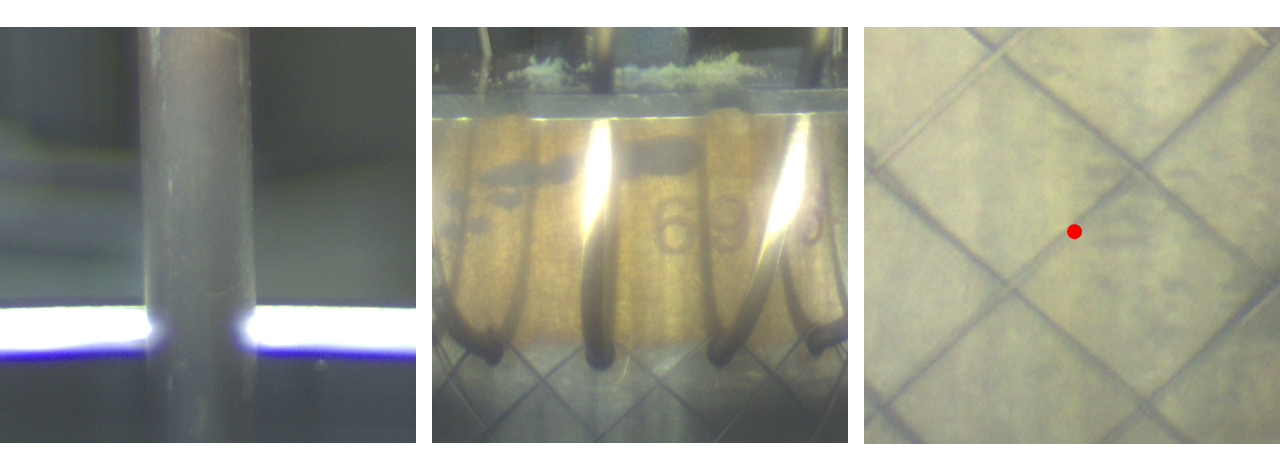
\includegraphics[width=12cm]{98_images/datensatz_bsp1.png}
\caption{Beispiele für ungeeignete Bilder für das neuronale Netz: kein Stent im Bild sichtbar (links), kein Pick in der Mitte des Bildes (Mitte), kein eindeutiger Pick in der Mitte (rot markiert) des Bildes (rechts). Bilder aus \cite{flechtmaschine} entnommen.}
\label{fig:datensatz-fehler-1}
\end{figure}

\mypar Zudem wurden im Anschluss weitere 11.150 Bilder aussortiert. Aufnahmen, bei denen die Lichtverhältnisse suboptimal waren, wurden entfernt, weil die Sichtbarkeit des mittleren Picks somit beeinflusst wurde und er nicht immer klar erkennbar war. Bilder von Stents, bei denen einer der Drähte gerissen war, wurden ebenfalls nicht übernommen. Abbildung \ref{fig:datensatz-fehler-2} zeigt drei Beispiele für die zuvor genannten Fälle. 

\begin{figure}[h!]
\centering
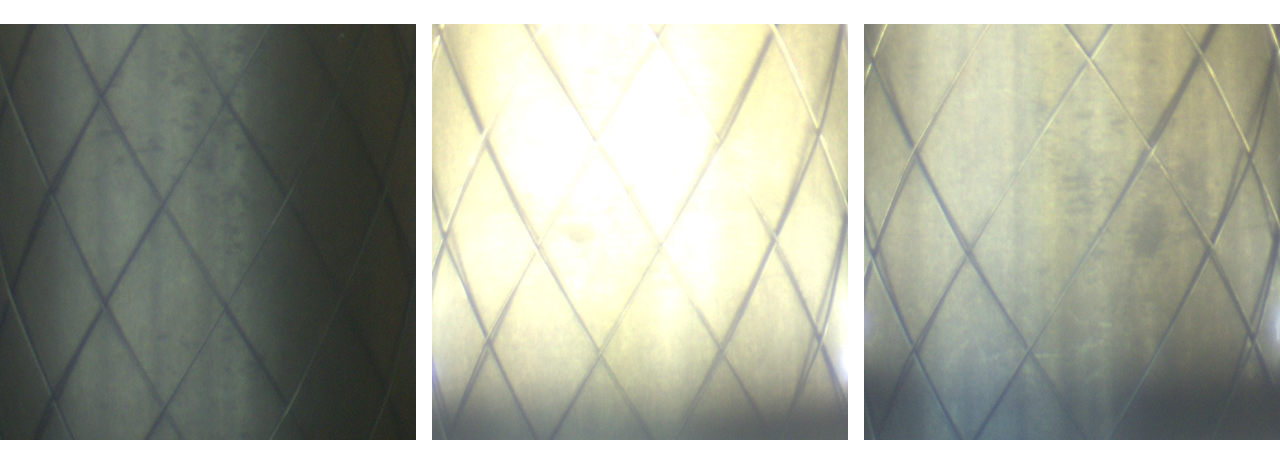
\includegraphics[width=12cm]{98_images/datensatz_bsp2.png}
\caption{Weitere Beispiele für aussortierte Bilder: ohne Licht (links), starke Lichtbestrahlung (Mitte), Draht gerissen (rechts). Bilder aus \cite{flechtmaschine} entnommen.}
\label{fig:datensatz-fehler-2}
\end{figure}

\mypar Nach dem Aussortieren ergab sich ein Datensatz mit 4.791 Bildern von Stents mit Flechtwinkeln von 30, 40, 50, 60 und 70 Grad. Tabelle \ref{Tab:Datensatz1} zeigt die Aufteilung der Anzahl an verwendbaren und aussortierten Bilddaten.

\begin{table}[h!]
\begin{center}
\begin{tabular}{cc}
Gesamte Bilder                & 23.527 \\ \hline
Ungeeignetes Licht            & 4.140  \\
Draht gerissen                & 7.010  \\
Kein Stent oder Pick sichtbar & 7.586  \\ \hline
Verwendbare Bilder            & 4.791 
\end{tabular}
\caption{Aufteilung der ursprünglichen Aufnahmen in verwendbare und ungeeignete Bilder}
\label{Tab:Datensatz1}
\end{center}
\end{table}

% Aufbereitung der Trainingsdaten
\section{Aufbereitung der Trainingsdaten}
Wie bereits beschrieben, konnten 4.791 geeignete Bilder aus den ursprünglichen Daten entnommen werden. Um den Datensatz zu erweitern, wurden diese verwendbaren Bilder durch das Drehen um 180° augmentiert. Da sich dadurch der zuvor markierte Pick aus dem Mittelpunkt des Bildes verschieben kann, wurde das Skript zum Labeln der Bilder erweitert. Somit konnten zuvor falsch gesetzte Labels gelöscht und Labels, bei denen sich der mittlere Pick nicht änderte für das augmentierte Bild übernommen werden. Hierdurch entstanden 3.892 weitere verwendbare Bilder inklusive Labels. Die Übersicht der Zusammensetzung des gesamten Datensatzes ist in Tabelle \ref{Tab:Trainingsdaten1} dargestellt.


\begin{table}[h!]
\begin{center}
\begin{tabular}{cc}
Datensatz             & Anzahl Bilder \\ \hline
Vorgeschnittene Daten & 4.791         \\
Augmentierte Daten    & 3.892         \\ \hline
Gesamter Datensatz    & 8.683        
\end{tabular}
\caption{Übersicht über die vorgeschnittenen, augmentierten und den daraus entstandenen gesamten Daten}
\label{Tab:Trainingsdaten1}
\end{center}
\end{table}

\mypar Eine detailliertere Darstellung vom Aufbau des Datensatzes wird durch Tabelle \ref{Tab:Trainingsdaten2} aufgezeigt. Es ist ersichtlich, dass keiner der Flechtwinkel einen mehrheitlichen Anteil des Datensatzes darstellt, wodurch eine Gleichverteilung der Flechtwinkel in den unterschiedlichen Datensätzen gewährleistet wird.. Im gesamten Datensatz betragen die kleinste und größte Picklänge 40,0 und 219,06 Pixel. Zudem entspricht ein Millimeter 23 Pixel in den Bildern. 

\begin{table}[h!]
\begin{center}
\begin{tabular}{l|l|l|l|l|l}
                       & 30 Grad & 40 Grad & 50 Grad & 60 Grad & 70 Grad \\ \hline
Vorgeschnittene Bilder & 880     & 1.142   & 988     & 878     & 903     \\
Augmentierte Bilder    & 816     & 974     & 845     & 657     & 600     \\ \hline
Gesamte Bilder         & 1696    & 2116    & 1833    & 1535    & 1503    \\
Prozentanteil          & 19,5    & 24,4    & 21,1    & 17,7    & 17,3   
\end{tabular}
\caption{Aufteilung der vorgeschnittenen und augmentierten Daten nach Flechtwinkel}
\label{Tab:Trainingsdaten2}
\end{center}
\end{table}


% Bildvorverarbeitung
\subsection{Bildvorverarbeitung}
Um die Erkennung gewisser Merkmale im Bild deutlicher zu machen, wurden die Bilder entsprechend vorverarbeitet. Hierfür wurde ein Histogrammausgleich durchgeführt, konkret der kontrastbegrenzte adaptive Histogrammausgleich aus Abschnitt \ref{sec:clahe-sec}. Die Implementierung wurde mit der Python-Bibliothek OpenCV \cite{bradski2000opencv} durchgeführt. Die Anwendung des gewöhnlichen Histogrammausgleichs, AHE und CLAHE aus Kapitel \ref{sec:histogramm-sec} wird in den Abbildungen \ref{fig:30grad-cropped-img}, \ref{fig:30grad-hist-eq-img}, \ref{fig:30grad-ahe-img} und \ref{fig:30grad-clahe-img} visualisiert.

\begin{figure}[ht]
\centering
\begin{minipage}[b]{0.45\linewidth}
    \centering
    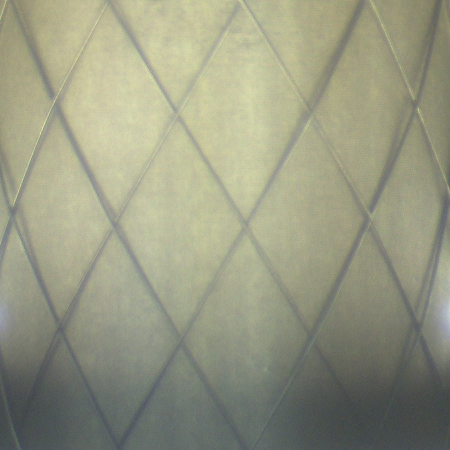
\includegraphics[width=4.5cm]{98_images/30grad_cropped.png}
    \caption{Ursprüngliches Bild}
    \label{fig:30grad-cropped-img}
\end{minipage}
\quad
\begin{minipage}[b]{0.45\linewidth}
    \centering
    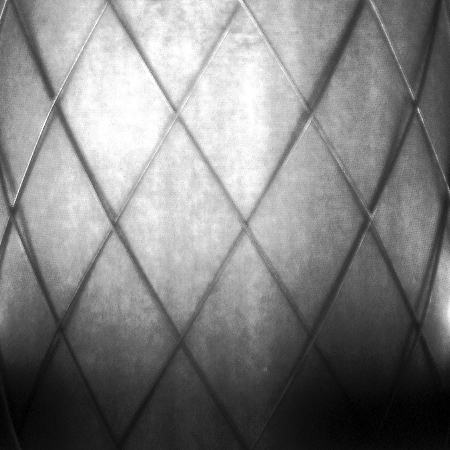
\includegraphics[width=4.5cm]{98_images/30grad_hist_eq.png}
    \caption{Histogrammausgleich}
    \label{fig:30grad-hist-eq-img}
\end{minipage}
\end{figure}

\begin{figure}[ht]
\centering
\begin{minipage}[b]{0.45\linewidth}
    \centering
    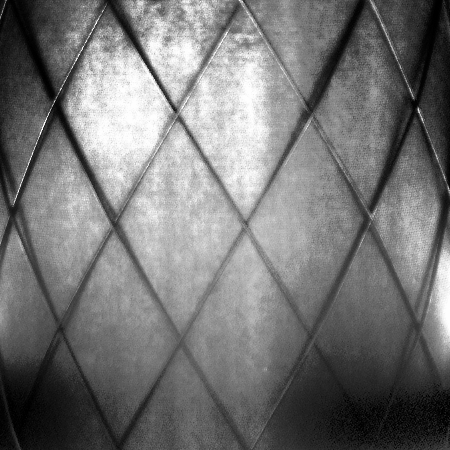
\includegraphics[width=4.5cm]{98_images/30grad_ahe.png}
    \caption{AHE}
    \label{fig:30grad-ahe-img}
\end{minipage}
\quad
\begin{minipage}[b]{0.45\linewidth}
    \centering
    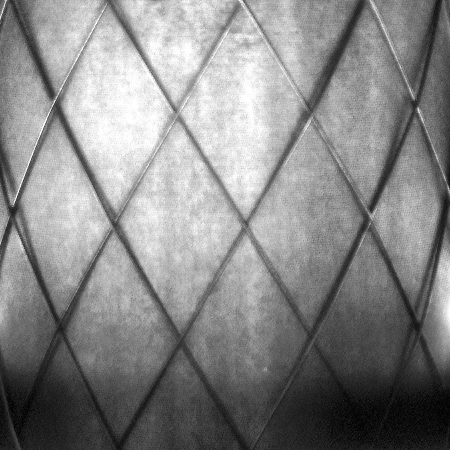
\includegraphics[width=4.5cm]{98_images/30grad_clahe.png}
    \caption{CLAHE}
    \label{fig:30grad-clahe-img}
\end{minipage}
\end{figure}


% Aufteilen und Normalisieren der Daten
\subsection{Aufteilen und Normalisieren der Daten}
Wie in Tabelle \ref{Tab:Trainingsdaten1} aufgezeigt, besteht der gesamte Datensatz aus 8.683 verwendbaren Bildern. Um die neuronalen Netze zu trainieren, werden ein Trainings- und ein Validierungsdatensatz benötigt. Zusätzlich ist ein Testdatensatz für die Evaluierung der einzelnen Netze notwendig. Aus diesem Grund wurde der Datensatz, wie in Tabelle \ref{Tab:train-val-test-tabelle} dargestellt, in drei kleinere Datensätze aufgeteilt. Dabei enthält der Trainingsdatensatz 70{\%} der Daten. Die Datensätze für die Validierung und das Testen bestehen jeweils aus 15{\%} der Bilder und Labels. 

\begin{table}[h!]
\begin{center}
\begin{tabular}{cc}
\textbf{Datensatz}   & \textbf{Anzahl Bilder} \\ \hline
Training    & 6.078         \\
Validierung & 1.302         \\
Test        & 1.303        
\end{tabular}
\caption{Aufteilung des gesamten Datensatzes in drei kleinere Datensätze}
\label{Tab:train-val-test-tabelle}
\end{center}
\end{table}

\mypar Wie in \cite{jo2019effectiveness} wurden die Daten anhand einer sogenannten Min-Max-Normalization zwischen den Werten Null und Eins gesetzt. Der MinMax-Scaler wurde erst auf den Inhalt des Trainingsdatesatzes angepasst und danach auf alle drei Datensätze angewendet. Um die Bilder und Labels aus diesen Datensätzen an die Netzwerkarchitekturen zu übergeben, wurde die Dataset API aus der Tensorflow-Bibliothek \cite{abadi2016tensorflow} verwendet, sodass eine Datenpipeline aufgebaut werden konnte.

\mypar Beim ersten Schritt wurden die Datensätze in TFRecord-Dateien umgewandelt. Dies hat den Vorteil, dass sie eine niedrigere Speicherkapazität benötigen und die Informationen der einzelnen Bilder zusammen mit ihren zugehörigen Labels hinterlegt werden. Zudem ist somit eine ununterbrochene Verbindung zum Laufwerk, auf dem die gesamten Daten gespeichert sind, nicht notwendig.

\mypar Um die Daten an den neuronalen Netzen zu übergeben, werden die einzelnen TFRecord-Dateien eingelesen. Mittels der Dataset API werden die eingelesenen Daten in einen Datensatz überführt. Danach werden die Bilder dekodiert und gecastet, um auf den Datentyp float32 umgewandelt zu werden. Die Werte der Labels werden ebenfalls auf den gleichen Datentyp umgewandelt. Im Anschluss wird der Datensatz aufgrund der Leistung des verwendeten Rechners in Batches der Größe acht aufgeteilt. Vorteil dieses Vorgehen ist, dass Bilder und Labels erst dekodiert und verarbeitet werden, wenn diese benötigt werden. 


% Faltende neuronale Netze
\section{Implementierung der faltenden neuronalen Netze}
Für die Implementierung der in Kapitel \ref{sec:auswahl-cnns} angedeuteten künstlichen faltenden neuronalen Netzen wurde die Tensorflow-Bibliothek mit der Keras API \cite{chollet2015keras} verwendet. Da mehrere der Modelle bereits in Keras eingebaut und auf dem ImageNet-Datensatz trainiert sind, konnten die vortrainierten Parameter übernommen werden. Dieser Vorgang wird als Transfer Learning gekennzeichnet und basiert auf der Prämisse, dass Menschen ihr vorher erlernetes Wissen anwenden können, um neue Probleme schneller und besser zu lösen; im Deep Learning funktioniert dies analog \cite{pan2009survey}.

\mypar Als Aktivierungsfunktion wurde die von der Veröffentlichung des Netzes vordefinierte Funktion verwendet. In Fällen, bei denen diese nicht vorgegeben war, wurde die Exponential Linear Unit (ELU) angewendet, da diese laut \cite{elus} nicht nur die Trainingszeit verkürzt, sondern die Leistung der Netze im Vergleich zur Anwendung von anderen Aktivierungsfunktionen wie ReLU verbessert. Zudem wurden alle drei in Kapitel \ref{sec:regularisierung-sec} beschriebenen Methoden der Regularisierung angewendet: Early Stopping, Dropout und L1L2-Regularisierung. Bei der Anwendung des Dropouts wurde die Rate aus den Veröffentlichungen, sofern diese vorgegeben war, übernommen. In den meisten Fällen war diese nicht angegeben, weshalb der Wert auf 0,5 gesetzt wurde. Laut Srivastava et al. \cite{dropout} ist diese Rate für eine breite Auswahl an Netzwerken und Aufgaben nahezu optimal. Für das Training der Netze wurde der Adam Optimierungsalgorithmus mit einer Anfangslernrate von $1 \cdot 10^{-6}$ gewählt. Zudem wurde das Mean Squared Error als Fehlerfunktion gewählt. 


% Reproduzierbarkeit
\section{Reproduzierbarkeit}
Im Rahmen des wissenschaftlichen Arbeitens ist die Reproduzierbarkeit eines der wichtigsten Prinzipien. Damit ist die Wiederholbarkeit bzw. Wiedererzeugbarkeit bestimmter Ergebnisse unter gleichen Umständen gemeint. Um dies zu ermöglichen, wurde ein sogenannter Seed verwendet. Dies ist ein beliebiger Wert, welcher Zufallsoperationen innerhalb des Codes steuert. Somit werden bei jeder Ausführung die gleichen drei Datensätze erstellt.

\mypar Für das Training der neuronalen Netze wurden zu Beginn die Seeds zur den Numpy-, Tensorflow- und Random-Bibliotheken gesetzt. Des Weiteren wurde die Seed auch zur Initialisierung der Parameter im Netz verwendet. Da im Vorgang des Trainings nicht nur die CPU, sondern auch die GPU des Rechners verwendet wird, kann dies zu Abweichungen bei der Ausführung des Codes führen. Hierdurch werden nämlich gewisse Bibliotheken der GPU verwendet, wodurch weitere Quellen für Zufallswerte eingeführt werden, welche nicht gesteuert werden können.


% Fehlerlokalisierung
\section{Fehlerlokalisierung}
Bezogen auf die Zielsetzung der Arbeit in Abschnitt \ref{sec:zielsetzung-sec}, soll eine Lokalisierung eines erkannten Fehlers im Anschluss möglich sein. Da die Lokalisierung einzelner Picks im Stent ein breites Thema ist, wurde dies nur oberflächlich untersucht. Deshalb wurde nur die Bestimmung eines Fehlers anhand eines Toleranzwertes untersucht. Es wurde ein kleines Programm geschrieben, welches eine willkürliche Anzahl an Bilder inklusive Labels und einen beliebigen Toleranzwert in Pixel entgegennimmt. Demnach werden die einzelnen Ausgaben des Netzes mit den Labels verglichen, um den Wert der Abweichung zu berechnen. Ist dieser Wert größer als die gesetzte Toleranz, wird die Abweichung in Pixel und der Pfad zum entsprechenden Bild in einer Ausgabedatei eingetragen. 




